\documentclass{article}
\usepackage{amsmath}
\usepackage{graphicx}
\usepackage{geometry}
\usepackage[hidelinks]{hyperref}
\geometry{
	a4paper,
	total={210mm,270mm},
	left=20mm,
	right=20mm,
	top=20mm,
	bottom=20mm}
\begin{document}
\title{Intership Project Status Report}
\maketitle
\section{Personal Details}
\textbf{Name:} Vijay G. Belurkar\\

\hspace{-5mm}\textbf{Email Id:} vijaybelurkar@gmail.com\\

\hspace{-5mm}\textbf{Department:} Electronics and Communication\\

\hspace{-5mm}\textbf{College:} PES Institute Of Technology, Bangalore\\

\hspace{-5mm}\textbf{Mobile Number:} +918147007507\\

\hspace{-5mm}\textbf{Title of Project:} Humanoid Robot\\

\hspace{-5mm}\textbf{Duration of the internship:} 26 May 2014 to 10 July 2014\\

\hspace{-5mm}\textbf{Summary of your contribution to the project:} The project assigned to my team was Humanoid Robot which was mentored by Saurav Shandilya and Vishwanathan Iyer under the guidance of Prof.Kavi Arya.\\
First of we identified that the project involved both Electronic as well as mechanical work and having a mechanical team member helped a lot. So we decided to split the work among us depending on our specialization. I had to basically do the embedded system part of the robot like interfacing and controlling the servo motors and troubleshooting when required. The programming part was handled by me to achieve all the basic motions of the robot. Since the given design had many faults we had to re-design the entire robot.The design and construction part was handled by both of us were we both brainstorm
the faults in the existing design and came up with the new design and build the whole structure together. 
\begin{center}
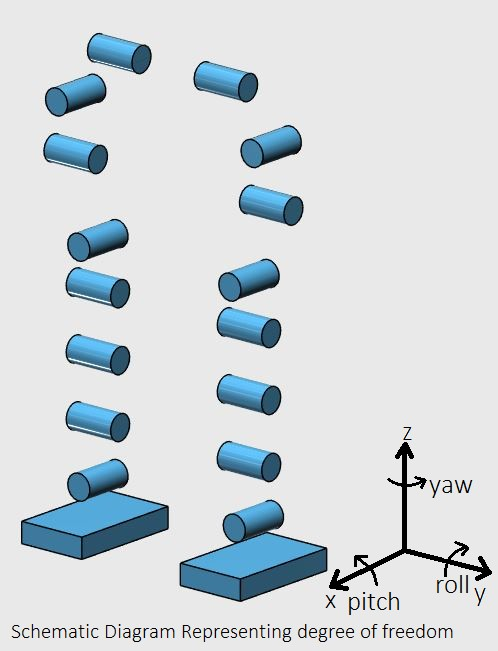
\includegraphics[width=6cm, height=8cm]{Schematic}
\end{center}
\newpage
\section{Project Status Report}
\textbf{Objective of the work:} I have always liked to work with hardwares rather than only programming stuff. So, I was inclined towards hardware projects given the list to us which involves automation using embedded programming.  \\
Our mentor initially instructed us that we have only concentrate on building a robust robot which can perform some basic moves and if time permitted we could do the advanced stuff like GUI,Camera etc\\
So,this was quite my kind of job and I choose to go with Humanoid Robot.\\

\hspace{-5mm}\textbf{Scope of the work:}Build a humanoid robot with 16 Degrees of Freedom and perform basic movements\\ 

\hspace{-5mm}\textbf{Completion:}Construction of Robot, Study Timers and Interrupts in ATMEGA 640, PWM generation using Interrupts, Interfacing Servo Motors, Calculation of the C.G, Sequence of servo for motion of the robot and design \& construction of the robot \\
\begin{center}
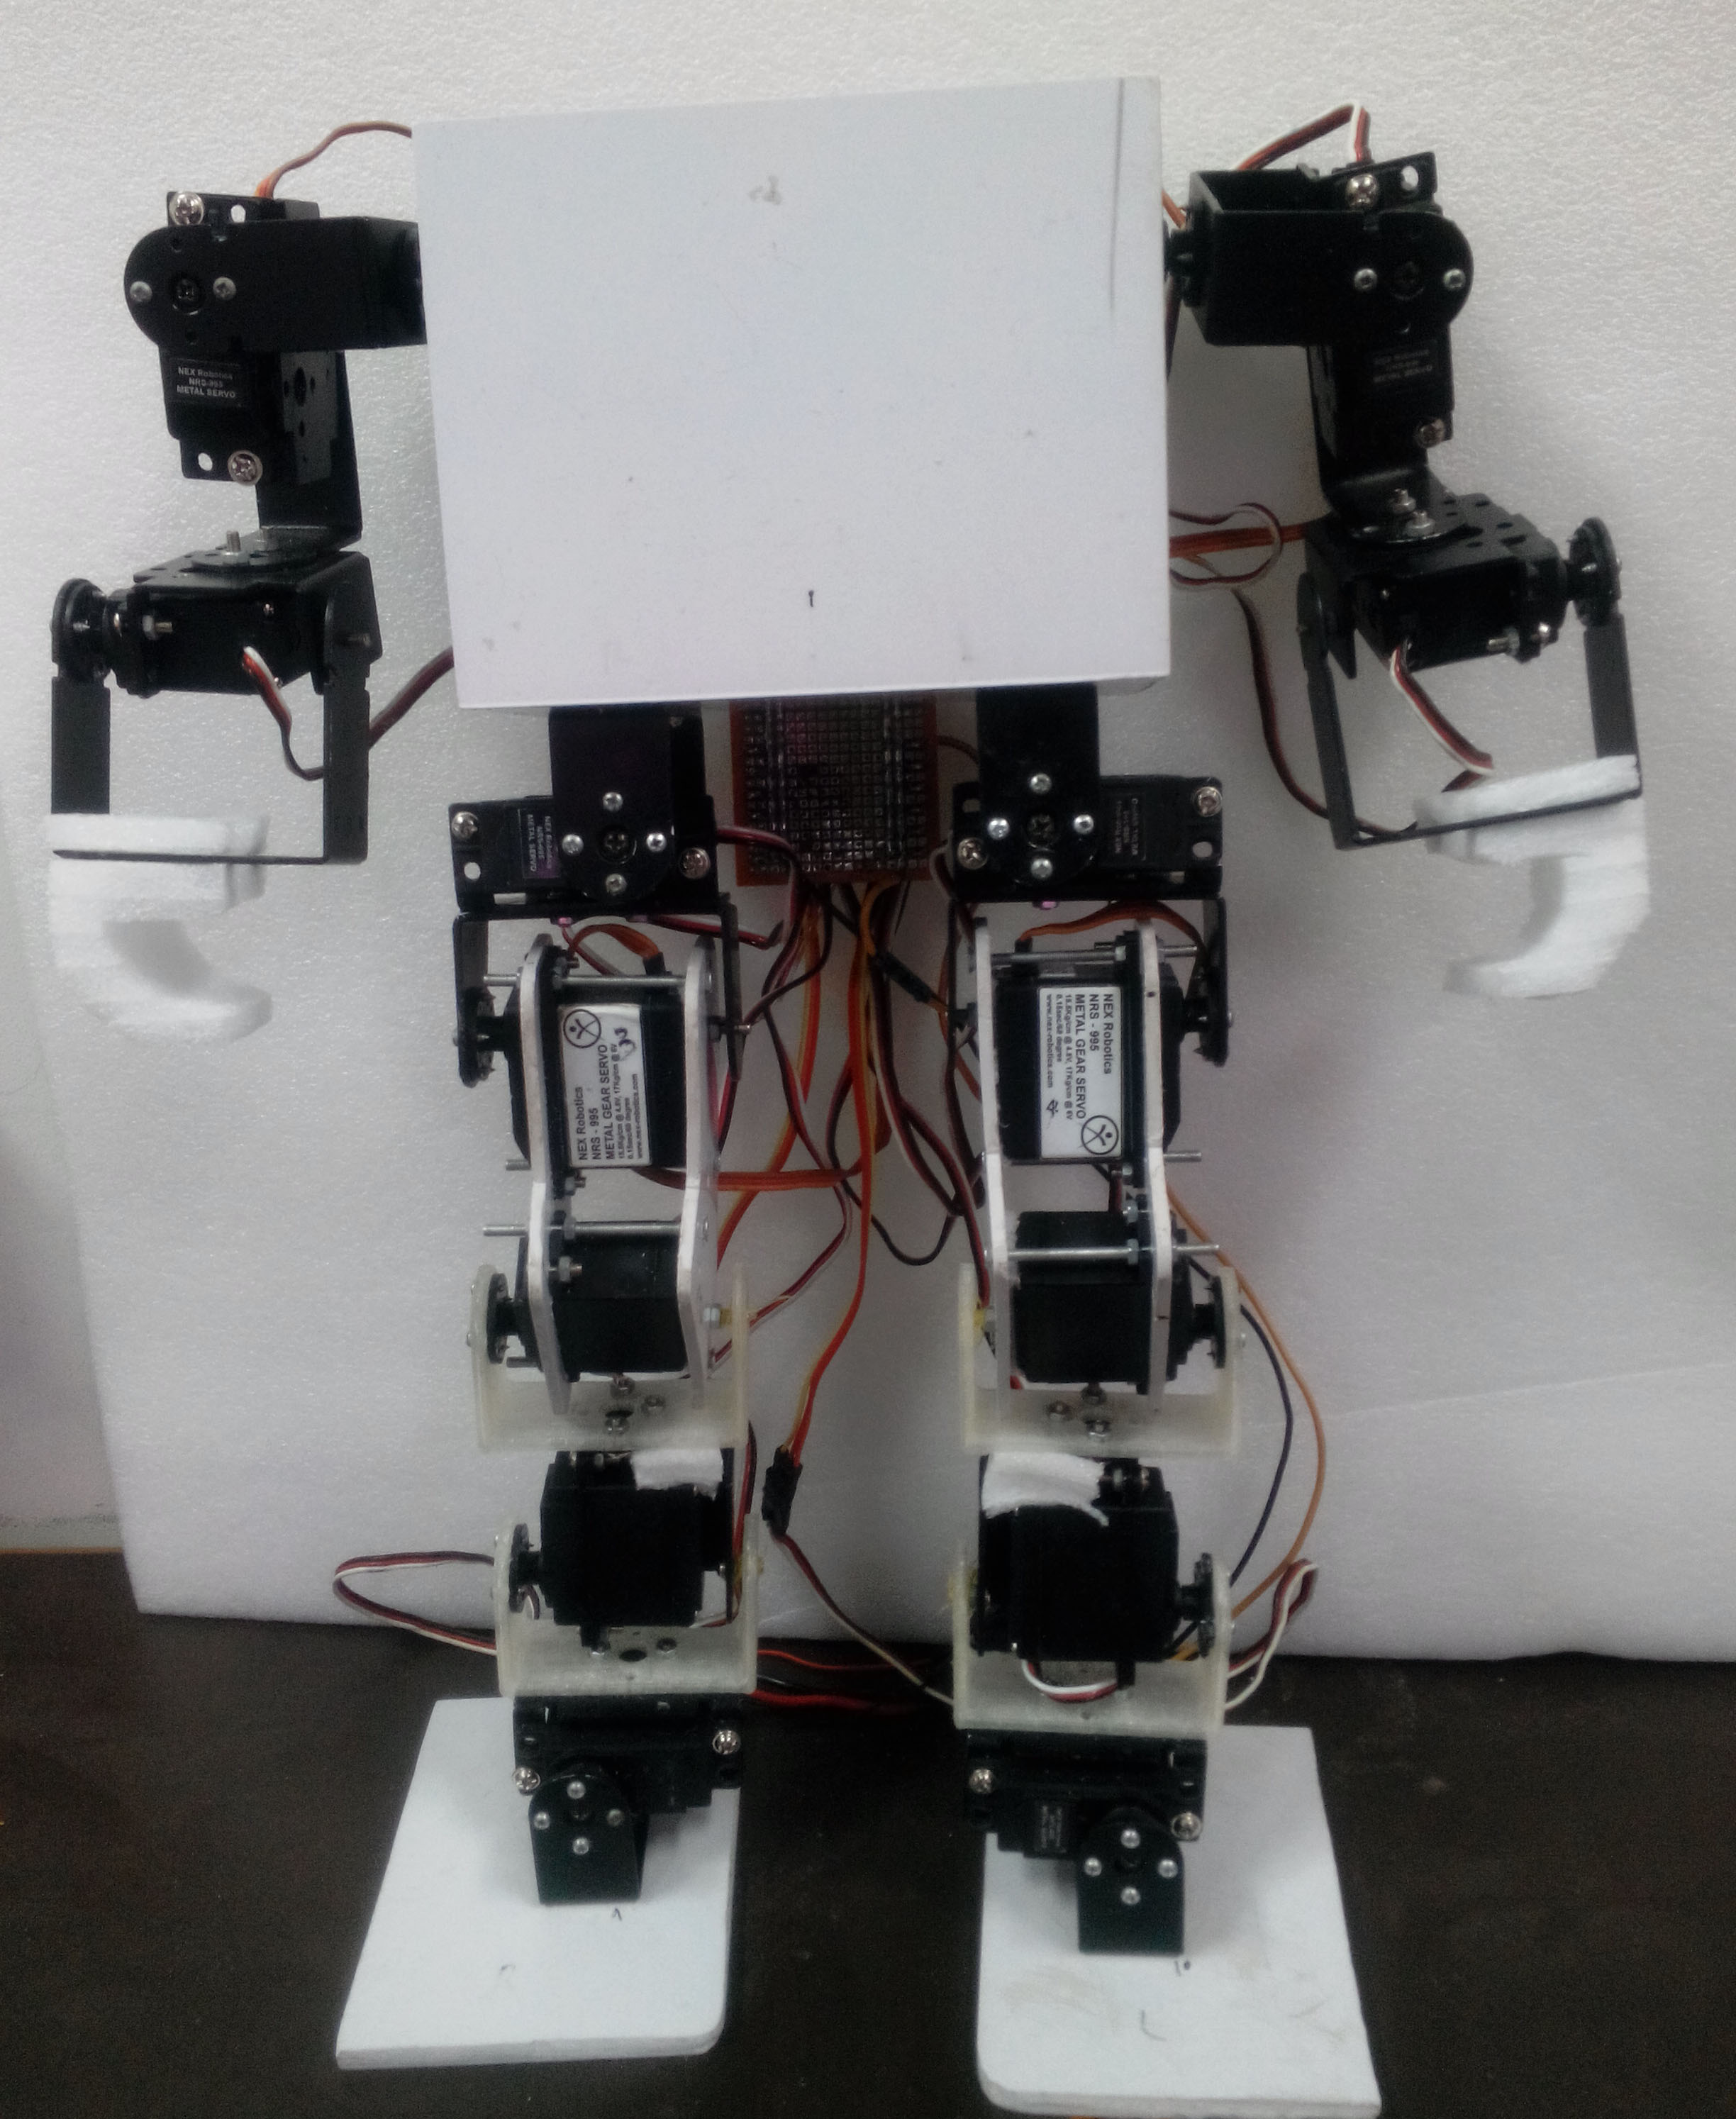
\includegraphics[width=6cm, height=8cm]{body_assembly}
\end{center}
\hspace{-5mm}\textbf{Results and Discussion:}We were successful in building a 16 DOFs humanoid which can walk, balance on one leg, do sit-ups. We had a choice of working on existing structure or build our own design from Scratch. We went with choice of working with the existing structure because it would save time, but we found many faults in the existing structure so we discarded that structure. Built our own structure simultaneously interfaced 16 servos on the micro-controller and calculated the C.G of the structure and then robot was programmed. Stability and motion of the robot was handled by me which involved calculation of C.G (center of gravity), describing the sequence of servos for motion of the robot both were completed successfully.          \\

\hspace{-5mm}\textbf{Features \& Bugs:}The features of the robot are, walk is human like, can balance on one leg, can perform sit-ups. Drawbacks are, existing structure cannot accommodate a battery on its body, and this can be fixed with little modification of the structure or the physical modification of the battery. Cannot walk on uneven surface  \\

\hspace{-5mm}\textbf{Future Work:}
\begin{enumerate}
	\item Making modules for different possible movements.
	\item Interfacing gyros for auto stabilization of the robot.
	\item Building a GUI for controlling the robot autonomously.
	\item Interfacing camera along with a smart processor like raspberry pi or a beagle board
	\item Interfacing various sensors like ultrasonic sensors for distance calculation, accelerometer,Xigbee for wireless communication.
\end{enumerate}
\begin{thebibliography}{99}
	\bibitem{zero} Zero-moment point method for stable biped walking\\
	DCT no.: 2009.072\\
	Internship report\\
	Eindhoven, July 2009.\\
	
	\bibitem{real} Real Time Biped Walking Gait Pattern Generator for a Real Robot\\
	Department of Computer Science and Technology,\\
	University of Science and Technology of China,\\
	Hefei, 230026, China\\
	
	\bibitem{design} Design and Implementation of a Simplified Humanoid Robot with 8 DOF\\
	Department of Electronics and Communication Engineering,\\ Hindustan Institute of
	Technology and Science,\\ Hindustan University, Chennai, India\\
	
	\bibitem{kin} Kinematics and Inverse Kinematics for the Humanoid Robot\\
	Rowland O’Flahertyy, Peter Vieiray, Michael Greyy,\\
	Paul Ohz, Aaron Bobicky, Magnus Egerstedty, and Mike Stilmany\\
	
	\bibitem{kinematics} Kinematics and Dynamics of a New 16 DOF Humanoid Biped Robot with Active Toe Joint\\
	Regular Paper\\
	C. Hernández-Santos, E. Rodriguez-Leal1, R. Soto1 and J.L. Gordillo\\
	
	
	\bibitem{robotic} Robotics (12 of Addis Ababa Lectures): Forward Kinematics of Spatial Robots\\
	\url{https://www.youtube.com/watch?v=NXWzk1toze4}\\
	
	\bibitem{robotic1}Robotics (1/3 of INGOU Lectures): An Introduction and Kinematic Configuration\\
	\url{https://www.youtube.com/watch?v=gNhK4VoV9P8}\\
	
	\bibitem{robotics2}Robotics (2/3 of IGNOU Lectures): Kinematics--Denavit and Hartenberg Parameters\\
	\url{https://www.youtube.com/watch?v=CnWTUsVle2A}\\
	
	\bibitem{robotics3}Robotics (3/3 of IGNOU Lectures): Forward and Inverse Kinematic Analyses\\
	\url{https://www.youtube.com/watch?v=duKD8cvtBTI}\\
	
	\bibitem{roboticswalk}Robot Basic Walk Tutorial\\
	\url{https://www.youtube.com/watch?v=Xhz6m6fu494}\\
	
\end{thebibliography}

\end{document}

